\section{Final remarks}

The following problem discussed in \cite[7.1]{AKP} was one of the original motivations to study the tree comparison.

\begin{thm}{Problem}
Which finite metric spaces admit isometric embeddings into some Alexandrov spaces with nonnegative curvature.
\end{thm}

The problem is still open.
According to \cite[4.1]{AKP}, the $(n-1)$-tree comparison provides a necessary condition for the problem $n$-point metric spaces.
This condition is sufficient for the 4-point metric spaces.
It might be still sufficient for 5-point metric spaces,
but not for 6-point metric spaces.

The corresponding example of 6-point metric space was constructed by Sergei Ivanov, see \cite{AKP}.
Theorem~\ref{2(2)+3(1)}, provides a source for such examples --- any 6-point metric space that satisfy all 5-tree comparisons, but does not satisfy 2(2)-tree comparison provides an example.
This class of examples includes the example of Sergei Ivanov --- in the notations of \cite[7.1]{AKP} it does not satisfies the comparison for the tree $y/az(q/xb)$.

By Theorem~\ref{2(2)+3(1)} and a theorem in \cite{AKP}, 
5-tree and 2(2)-tree comparisons provide a necessary condition for 6-point metric spaces.
We expect that these conditions are sufficient

\begin{center}
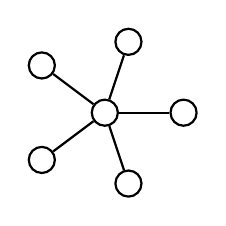
\begin{tikzpicture}[scale=1,
  thick,main node/.style={circle,draw,font=\sffamily\bfseries,minimum size=3mm}]

  \node[main node] (1) at (.3,-.9) {};
  \node[main node] (2) at (0,0){};
  \node[main node] (3) at (.3,.9){};
  \node[main node] (4) at (1,0) {};
  \node[main node] (5) at (-.8,-.6) {};
  \node[main node] (6) at (-.8,.6) {};

  \path[every node/.style={font=\sffamily\small}]
   (1) edge node[above]{}(2)
   (2) edge node[above]{}(3)
   (2) edge node[above]{}(4)
   (2) edge node[above]{}(5)
   (2) edge node[above]{}(6);
\end{tikzpicture}
\hskip30mm
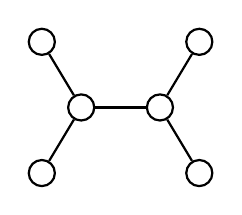
\begin{tikzpicture}[scale=1,
  thick,main node/.style={circle,draw,font=\sffamily\bfseries,minimum size=3mm}]

  \node[main node] (1) at (0,0) {};
  \node[main node] (2) at (1/2,5/6){};
  \node[main node] (3) at (0,10/6){};
  \node[main node] (4) at (2,0) {};
  \node[main node] (5) at (3/2,5/6) {};
  \node[main node] (6) at (2,10/6) {};

  \path[every node/.style={font=\sffamily\small}]
   (1) edge node[above]{}(2)
   (2) edge node[above]{}(3)
   (2) edge node[above]{}(5)
   (4) edge node[above]{}(5)
   (5) edge node[above]{}(6);
\end{tikzpicture}

\end{center}

Here an other candidate for a sufficient condition.

\begin{thm}{Question}
Assume $F$ is a finite metric space that satisfies all tree comparisons.
Is it true that $F$ is isometric to a subset of an Alexandrov space with nonnegative curvature?
\end{thm}

Note that even for finite metric space the all tree comparison has to be checked for an infinite set of trees since one point of the space may be used as a label for several vertexes in the tree.

There is a chance that for 5-point and 6-point metric spaces, this condition is also necessary. 
Since there are nonnegatively curved Riemannian manifolds that are not cost-convex, 
Theorem~\ref{T=>CTIL:CTIL} implies that this condition can not be necessary for 7-point metric spaces.

\medskip

For any metric space $X$ with an isometric group action $G\acts X$ with closed orbits the quotient map $X\to X/G$ is a submetry.
In particular, by Theorem~\ref{thm:hilbert-quotient}, if $G\acts \HH$ is an isometric action with closed orbits on the Hilbert space, then the quotient space $\HH/G$ satisfies all tree comparisons.

\begin{thm}{Question}
Assume $X$ is a metric space satisfying all tree comparisons.
Is it always possible to construct an isometric group action with closed orbits on the Hilbert space $G\acts \HH$ such that $X$ is isometric to a subset in $\HH/G$?
\end{thm}